\documentclass[french,a4paper,10pt]{article}
% pdflatex compte_rendu.tex -output-directory=out && mv out/compte_rendu.pdf ./

\usepackage[a4paper,hmargin=30mm,vmargin=30mm]{geometry}
\usepackage[T1]{fontenc} % font type
\usepackage[french]{babel} % language
\usepackage{lmodern} % font type
\usepackage[shortlabels]{enumitem}
\usepackage{hyperref}
\usepackage{graphicx}
\usepackage{sectsty}
\usepackage{amsmath}
%\setlength{\parindent}{0pt}



\title{Compte Rendu TP5\\
Traitement d'images en couleur\\
Changement d'espaces couleur}
\author{Ivan Lejeune}
\date{\today}


\begin{document}
    \maketitle

    % make table of contents
    \tableofcontents

    \newpage
    \section{Obtention d'une image en niveaux de gris à partir d'une image couleur}\label{sec:1}

    \subsection{Choix de l'image}\label{subsec:1.1}

    Comme lors des TP précédents, on utilise l'image \texttt{peppers.ppm} et
    \texttt{peppers.pgm} pour les tests.

    % insert both images
    \begin{figure}[!htb]
        \begin{minipage}{0.48\textwidth}
            \centering
            \fbox{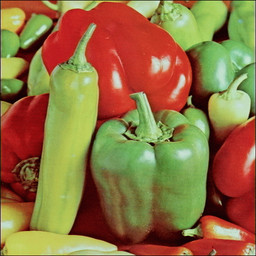
\includegraphics[width=.7\linewidth]{./out/orig-peppers}}
            \caption{Image originale}\label{Fig:orig-peppers}
        \end{minipage}\hfill
        \begin{minipage}{0.48\textwidth}
            \centering
            \fbox{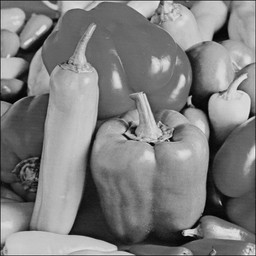
\includegraphics[width=.7\linewidth]{./out/peppers-grey}}
            \caption{Image en niveaux de gris}\label{Fig:peppers-grey}
        \end{minipage}
    \end{figure}

    \subsection{Transformation de l'image en niveaux de gris}\label{subsec:1.2}

    On commence par écrire le programme \texttt{RGB\_to\_Y} qui prend en entrée
    une image couleur et renvoie une image en niveaux de gris.
    Pour cela, on utilise la formule suivante :
    \[
        Y = 0.299 \cdot R + 0.587 \cdot G + 0.114 \cdot B
    \]

    On obtient alors les résultats suivants :
    % insert peppers-grey and rgb-to-y-peppers
    \begin{figure}[!htb]
        \begin{minipage}{0.48\textwidth}
            \centering
            \fbox{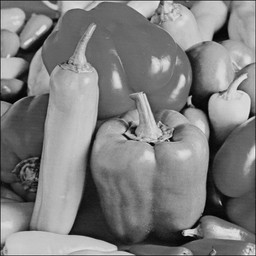
\includegraphics[width=.7\linewidth]{./out/peppers-grey}}
            \caption{Image en niveaux de gris}\label{Fig:peppers-grey-1}
        \end{minipage}\hfill
        \begin{minipage}{0.48\textwidth}
            \centering
            \fbox{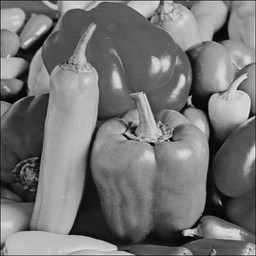
\includegraphics[width=.7\linewidth]{./out/peppers_rgb-to-y}}
            \caption{Image obtenue avec \texttt{RGB\_to\_Y}}\label{Fig:peppers_rgb-to-y}
        \end{minipage}
    \end{figure}

    \newpage

    \subsection{Comparaison des deux images}\label{subsec:1.3}

    On compare les deux images obtenues en calculant l'erreur quadratique moyenne
    (EQM) avec la formule suivante :
    \[
        EQM = \frac{1}{n} \sum_{i=1}^{n} (Y_i - Y'_i)^2
    \]

    Où $Y_i$ est la valeur du pixel $i$ de l'image originale et $Y'_i$ est la
    valeur du pixel $i$ de l'image obtenue.

    On obtient alors l'EQM suivante :
    \[
        EQM = 113.847305
    \]

    \newpage
    \section{Transformation de l'espace RGB vers l'espace YCbCr}\label{sec:2}

    \subsection{Programme}\label{subsec:2.1}

    On commence par écrire le programme \texttt{RGB\_to\_YCbCr} qui prend en
    entrée une image couleur et renvoie 3 images en niveaux de gris correspondant
    aux composantes Y, Cb et Cr de l'image originale.

    On utilise les formules suivantes :
    \[\begin{aligned}
            Y &= 0.299 \cdot R + 0.587 \cdot G + 0.114 \cdot B \\
            Cb &= 128 - 0.1687 \cdot R - 0.3313 \cdot G + 0.5 \cdot B \\
            Cr &= 128 + 0.5 \cdot R - 0.4187 \cdot G - 0.0813 \cdot B
    \end{aligned}\]

    On obtient alors les résultats suivants :
    % insert peppers-y, peppers-cb, peppers-cr
    \begin{figure}[!htb]
        \begin{minipage}{0.3\textwidth}
            \centering
            \fbox{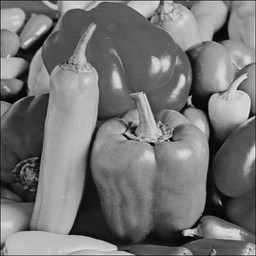
\includegraphics[width=.7\linewidth]{./out/peppers_Y}}
            \caption{Composante Y}\label{Fig:peppers_y}
        \end{minipage}\hfill
        \begin{minipage}{0.3\textwidth}
            \centering
            \fbox{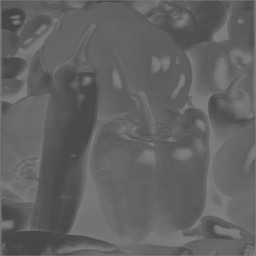
\includegraphics[width=.7\linewidth]{./out/peppers_Cb}}
            \caption{Composante Cb}\label{Fig:peppers_cb}
        \end{minipage}\hfill
        \begin{minipage}{0.3\textwidth}
            \centering
            \fbox{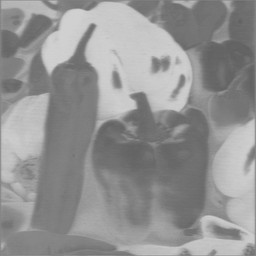
\includegraphics[width=.7\linewidth]{./out/peppers_Cr}}
            \caption{Composante Cr}\label{Fig:peppers_cr}
        \end{minipage}
    \end{figure}

    \newpage

    \section{Transformation de l'espace YCbCr vers l'espace RGB}\label{sec:3}

    \subsection{Programme}\label{subsec:3.1}

    On commence par écrire le programme \texttt{YCbCr\_to\_RGB} qui prend en
    entrée 3 images en niveaux de gris correspondant aux composantes Y, Cb et Cr
    d'une image couleur et renvoie l'image couleur originale.

    On utilise les formules suivantes :
    \[\begin{aligned}
            R &= Y + 1.402 \cdot (Cr - 128) \\
            G &= Y - 0.34414 \cdot (Cb - 128) - 0.714414 \cdot (Cr - 128) \\
            B &= Y + 1.772 \cdot (Cb - 128)
    \end{aligned}\]

    On obtient alors les résultats suivants :
    % insert orig-peppers and peppers-rgb
    \begin{figure}[!htb]
        \begin{minipage}{0.48\textwidth}
            \centering
            \fbox{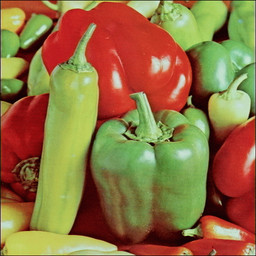
\includegraphics[width=.7\linewidth]{./out/orig-peppers}}
            \caption{Image originale}\label{Fig:orig-peppers-2}
        \end{minipage}\hfill
        \begin{minipage}{0.48\textwidth}
            \centering
            \fbox{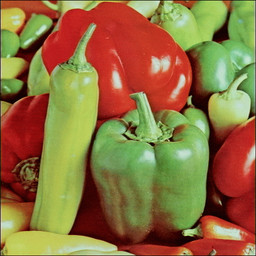
\includegraphics[width=.7\linewidth]{./out/peppers_YCbCr-to-rgb}}
            \caption{Image obtenue avec \texttt{YCbCr\_to\_RGB}}\label{Fig:peppers_YCbCr-to-rgb}
        \end{minipage}
    \end{figure}

    \newpage
    \section{Inversion de composantes à la reconstruction}\label{sec:4}

    \subsection{Programme}\label{subsec:4.1}

    On commence par écrire le programme \texttt{YCbCr\_to\_mix\_RGB} qui
    prend en entrée 3 images en niveaux de gris correspondant aux composantes Y,
    Cb et Cr d'une image couleur et renvoie 6 images correspondant à toutes les
    combinaisons possibles des composantes Y, Cb et Cr.

    On obtient alors les résultats suivants :
    % insert images as triplets, two times, outputof the modified images being
    % names peppers-YRGB, peppers-YRBG etc
    \begin{figure}[!htb]
        \begin{minipage}{0.3\textwidth}
            \centering
            \fbox{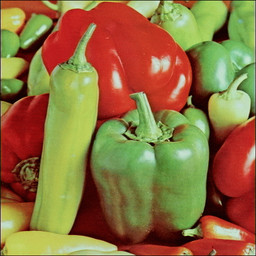
\includegraphics[width=.7\linewidth]{./out/peppers_mix-RGB}}
            \caption{Composantes dans l'ordre RGB}\label{Fig:peppers_mix-RGB}
        \end{minipage}\hfill
        \begin{minipage}{0.3\textwidth}
            \centering
            \fbox{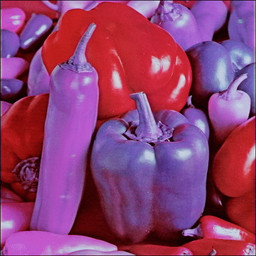
\includegraphics[width=.7\linewidth]{./out/peppers_mix-RBG}}
            \caption{Composantes dans l'ordre RBG}\label{Fig:peppers_mix-RBG}
        \end{minipage}\hfill
        \begin{minipage}{0.3\textwidth}
            \centering
            \fbox{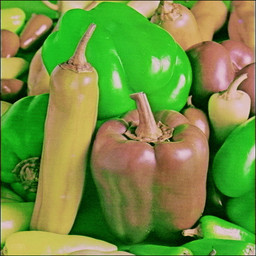
\includegraphics[width=.7\linewidth]{./out/peppers_mix-GRB}}
            \caption{Composantes dans l'ordre GRB}\label{Fig:peppers_mix-GRB}
        \end{minipage}
    \end{figure}

    \begin{figure}[!htb]
        \begin{minipage}{0.3\textwidth}
            \centering
            \fbox{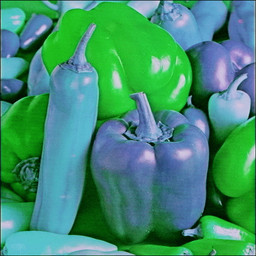
\includegraphics[width=.7\linewidth]{./out/peppers_mix-BRG}}
            \caption{Composantes dans l'ordre BRG}\label{Fig:peppers_mix-BRG}
        \end{minipage}\hfill
        \begin{minipage}{0.3\textwidth}
            \centering
            \fbox{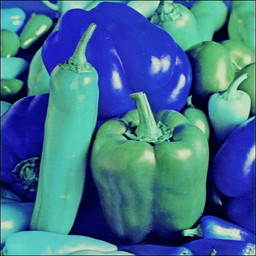
\includegraphics[width=.7\linewidth]{./out/peppers_mix-BGR}}
            \caption{Composantes dans l'ordre BGR}\label{Fig:peppers_mix-BGR}
        \end{minipage}\hfill
        \begin{minipage}{0.3\textwidth}
            \centering
            \fbox{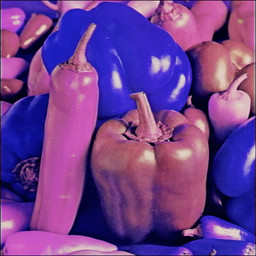
\includegraphics[width=.7\linewidth]{./out/peppers_mix-GBR}}
            \caption{Composantes dans l'ordre GBR}\label{Fig:peppers_mix-GBR}
        \end{minipage}
    \end{figure}

    \newpage

    \section{Modification de la luminance d'une image couleur}\label{sec:5}

    \subsection{Programme}\label{subsec:5.1}

    On commence par écrire le programme \texttt{modify\_luminance} qui prend en
    entrée la composante Y d'une image couleur et un entier $k$ et renvoie une
    image grise correspondant à la composante Y multipliée par $k$.

    On obtient alors les résultats suivants :
    % insert peppersY-modif-'k' with k = 10, 50, -30
    \begin{figure}[!htb]
        \begin{minipage}{0.3\textwidth}
            \centering
            \fbox{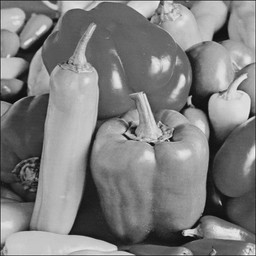
\includegraphics[width=.7\linewidth]{./out/peppers-modif-10}}
            \caption{image modifiée par 10}\label{Fig:peppersY-modif-10}
        \end{minipage}\hfill
        \begin{minipage}{0.3\textwidth}
            \centering
            \fbox{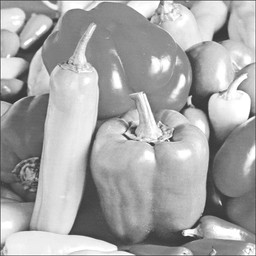
\includegraphics[width=.7\linewidth]{./out/peppers-modif-50}}
            \caption{image modifiée par 50}\label{Fig:peppersY-modif-50}
        \end{minipage}\hfill
        \begin{minipage}{0.3\textwidth}
            \centering
            \fbox{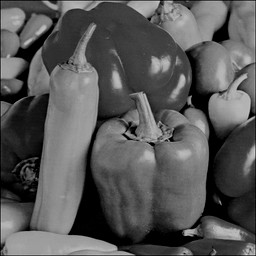
\includegraphics[width=.7\linewidth]{./out/peppers-modif--30}}
            \caption{image modifiée par -30}\label{Fig:peppersY-modif--30}
        \end{minipage}
    \end{figure}

    \newpage

    \subsection{Comparaison des images}\label{subsec:5.2}

    On choisit d'utiliser l'image modifiée par -30 pour la comparaison.
    Les résultats sont les suivants :

    \begin{figure}[!htb]
        \begin{minipage}{0.48\textwidth}
            \centering
            \fbox{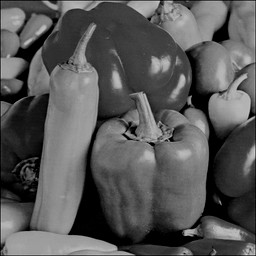
\includegraphics[width=.7\linewidth]{./out/peppers-modif--30}}
            \caption{image modifiée par -30}\label{Fig:peppersY-modif--30-2}
        \end{minipage}\hfill
        \begin{minipage}{0.48\textwidth}
            \centering
            \fbox{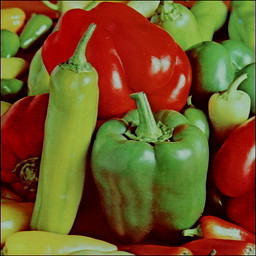
\includegraphics[width=.7\linewidth]{./out/peppers_YCbCr-to-rgb-modif--30}}
            \caption{Image obtenue avec \texttt{YCbCr\_to\_RGB}}\label{Fig:peppers_YCbCr-to-rgb-modif--30}
        \end{minipage}
    \end{figure}

    \subsection{Comparaison des histogrammes}\label{subsec:5.3}

    On compare les histogrammes des images \texttt{peppers.ppm} et
    \texttt{peppers-modif--30.ppm}.
    Les résultats sont les suivants :

    \begin{figure}[!htb]
        \centering
        \fbox{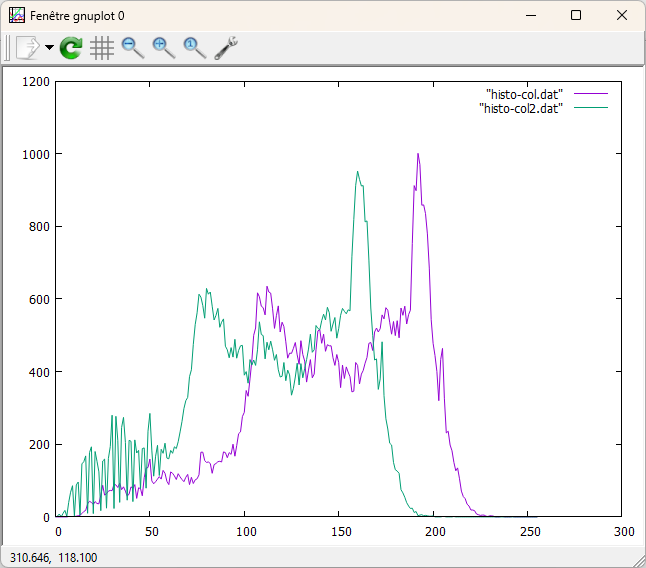
\includegraphics[width=.7\linewidth]{./out/histo-peppers-luminance}}
        \caption{Histogramme de \texttt{peppers.ppm}}\label{Fig:histo-peppers-luminance}
    \end{figure}

\end{document}